\section{Introducción a tipos sesión}

\begin{frame}{\insertsection}

	El desarrollo de software distribuido se enfoca principalmente en la
	integración, cooperación y comunicación de componentes en un sistema.

	\bigskip

	Dificultades:
	\begin{itemize}
		\item{Desafío tecnológico}
		\item{\alert<2>{Razonamiento sobre el sistema}}
		\pause
	\end{itemize}

	\note{Primero introducción a qué son y
	qué problema buscan resolver los tipos sesión. Después charlar sobre la
	variante probabilística. Luego el objetivo de este trabajo y un paseo
	por el mismo.}
	\note{Desafío tecnológico: trabajo correspondiente a la
	integración concreta de los componentes. Implementación.
	\\
	Razonamiento: comprender el estado de un sistema distribuido.}
\end{frame}

\begin{frame}{\insertsection}
	\begin{figure}
		\centering
		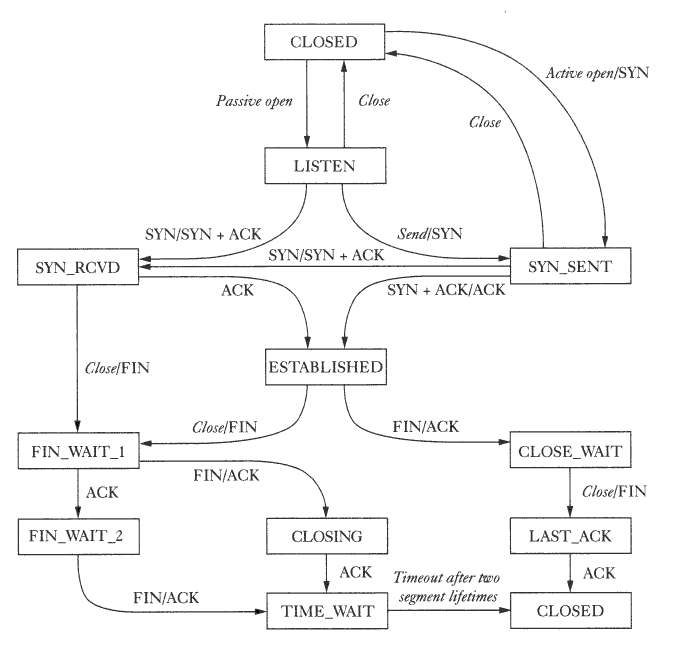
\includegraphics[width=0.6\textwidth]{images/tcp-state-diagram.png}
		\caption{Diagrama de estados para protocolo \textsc{TCP}}
	\end{figure}
	\note{Mostrar brevemente como ejemplo de la complejidad que puede tener un sistema distribuido en términos de estados posibles y propiedades a lo largo de los mismos}
\end{frame}

\begin{frame}{\insertsection}

	Esto dio lugar a:

	\begin{itemize}
		\item Desarrollo de técnicas de descripción de interfaces
		\item Soporte a nivel de lenguajes de programación para el desarrollo de aplicaciones correctas por construcción
	\end{itemize}

	\pause

	Los tipos comportamentales, tales como los \textbf{tipos de sesión} constituyen
	un ejemplo paradigmático de esta línea de trabajo.
\end{frame}

\begin{frame}{\insertsection}
	Los tipos de sesión proponen estructurar la
	comunicación entre componentes alrededor del concepto de \textbf{sesión}.

	\begin{itemize}
		\item Una sesión es un canal privado que permite
			conectar a dos (a veces más) procesos.

		\item Cada proceso posee un \textbf{endpoint} de la sesión y lo
			debe usar siguiendo un protocolo bien especificado
			(tipo sesión) que restringe la secuencia de mensajes
			que se pueden enviar y recibir a través del mismo.
	\end{itemize}

	\begin{figure}
		\centering
		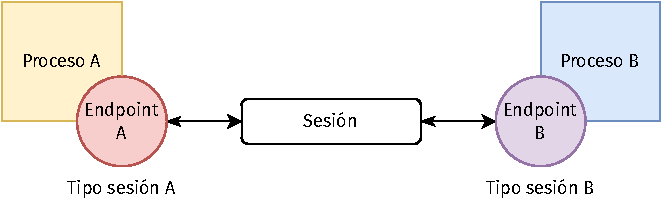
\includegraphics[width=0.8\textwidth]{images/tipo-sesion.pdf}
		\caption{Estructura de comunicación mediante tipos sesión}
	\end{figure}
\end{frame}

\subsection{Ejemplo: Describiendo suma con tipos sesión}

\begin{frame}{\insertsubsection}
	Consideremos un protocolo básico para la suma de dos números:
	\begin{enumerate}
		\item Cliente envía primer sumando
		\item Cliente envía segundo sumando
		\item Servidor retorna suma
	\end{enumerate}
\end{frame}

\begin{frame}{\insertsubsection}
	\begin{figure}
		\centering
		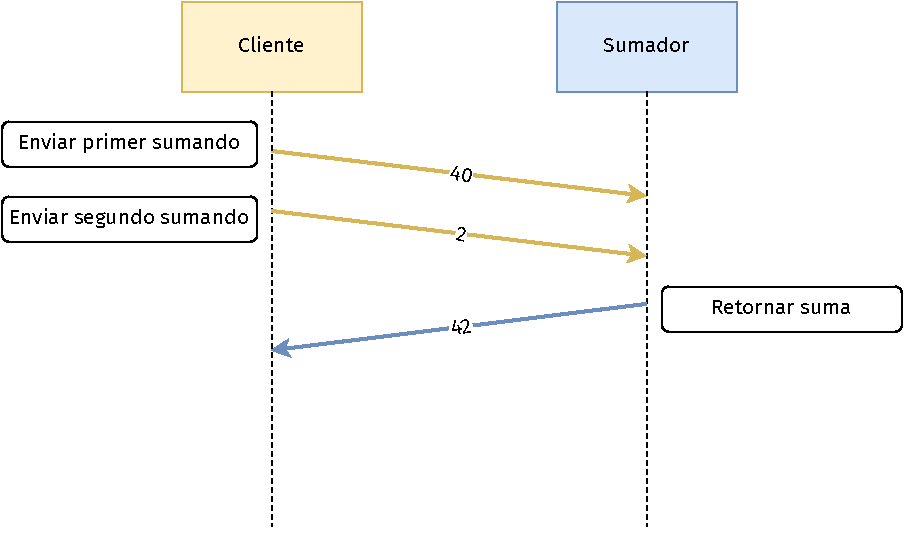
\includegraphics[width=0.9\textwidth]{images/sum-diagram.pdf}
		\caption{Ejemplo de comunicación para servicio sumador}
	\end{figure}
\end{frame}

\begin{frame}{\insertsubsection}
	\begin{figure}
		\centering
		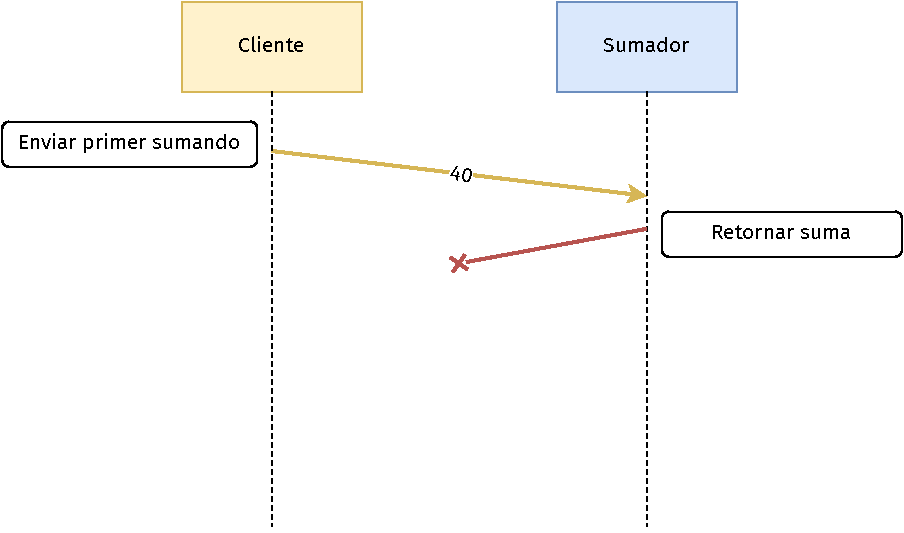
\includegraphics[width=0.9\textwidth]{images/sum-diagram-illegal.pdf}
		\caption{Violación de linearidad}
	\end{figure}
\end{frame}

\begin{frame}{\insertsubsection}
	\begin{figure}
		\centering
		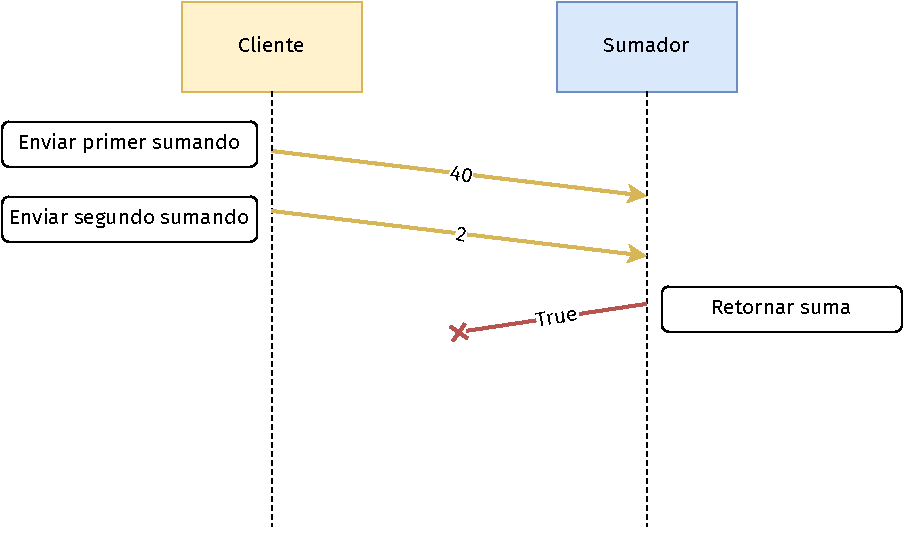
\includegraphics[width=0.9\textwidth]{images/sum-diagram-type-violation.pdf}
		\caption{Tipo de valor de retorno inválido}
	\end{figure}
\end{frame}

\begin{frame}{\insertsubsection}
	Para este ejemplo, la comunicación podría estructurarse mediante los siguientes tipos sesión:
	\begin{itemize}
		\item \textbf{Cliente:} $\SessionType = \Out\tint{ \Out\tint{ \In\tint\End } }$
		\item \textbf{Sumador:} $\dual\SessionType = \In\tint{ \In\tint{ \Out\tint\End } }$
	\end{itemize}

	\begin{figure}
		\centering
		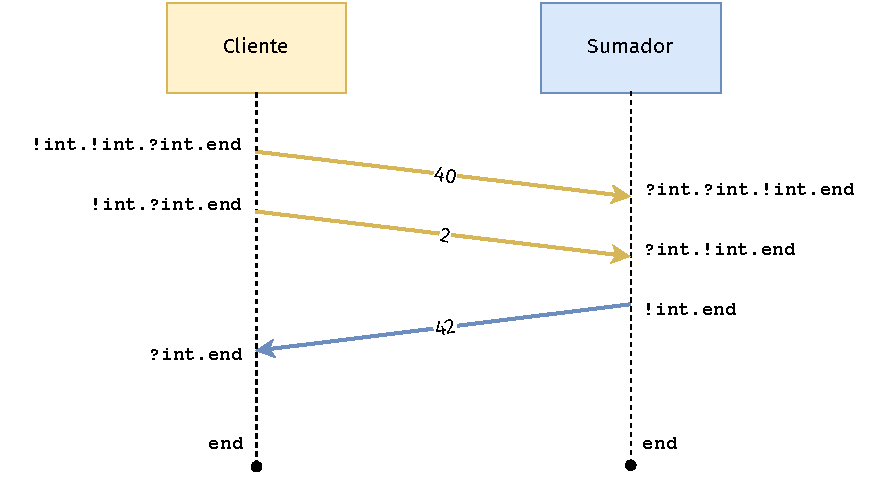
\includegraphics[width=0.9\textwidth]{images/sum-diagram-st.pdf}
	\end{figure}
\end{frame}

\subsection{Implementación de tipos sesión: FuSe}

\begin{frame}{\insertsubsection}
	\FuSe \footfullcite{DBLP:journals/jfp/Padovani17} es una biblioteca que habilita el uso de tipos sesión binarios en
	\OCaml.
	\begin{itemize}
		\item Codificación basada en igualdad de tipos y tipos parametrizados.
		\item Detección de violaciones de linearidad en tiempo de ejecución.
		\item Garantiza comunicación segura, fidelidad y progreso (siempre y cuando no haya deadlocks y se respete la linearidad).
		\item Inferencia de tipos y subtipado provisto por el sistema de tipos de \OCaml.
	\end{itemize}
	\begin{figure}
		\centering
		
\includegraphics[width=0.3\textwidth]{images/ocaml-logo.png}
	\end{figure}
\end{frame}

\begin{frame}{\insertsubsection}
	\SumClient
	Evolución del tipo sesión:
	\begin{itemize}
		\item \OI{ep0:} $\Out\tint{ \Out\tint{ \In\tint\End } }$
		\item \OI{ep1:} $\Out\tint{ \In\tint\End }$
		\item \OI{ep2:} $\In\tint\End$
		\item \OI{ep3:} $\End$
	\end{itemize}
\end{frame}

\begin{frame}{\insertsubsection}
	\SumServer
	Creamos un \emph{thread} con el sumador y realizamos una suma con el cliente:
	\SumExample
\end{frame}

\subsection{Elecciones}

\begin{frame}{\insertsubsection}
	Además de enviar y recibir, un protocolo puede presentar bifurcaciones,
	elecciones que impacten en cómo se desarrolla el mismo.

	\SumServerRec

	Donde \OI{ep0} es un endpoint de tipo sesión: $\SessionType = \In\tint{ \In\tint{
		\Out\tint\BinaryPBranch[]\T\End } }$
\end{frame}

\begin{frame}{\insertsubsection}
	\SumThreeNumClient
	Donde \OI{ep0} es un endpoint de tipo sesión: $\dual\SessionType = \Out\tint{ \Out\tint{
		\In\tint{\Choice\set{\Tag[True]: \Out\tint{ \Out\tint{
		\In\tint{\Choice\set{\Tag[False]: \End} }}}} }}}$
\end{frame}

\section{Tipos sesión probabilísticos}

\begin{frame}{\insertsection: Subasta}
	En \emph{``Probabilistic Analysis of Binary Sessions''}\footfullcite{DBLP:conf/concur/InversoMPTT20} se propuso el uso de tipos de sesión
	para razonar probabilísticamente sobre propiedades de alcanzabilidad,
	donde se dio una interpretación \emph{probabilística} a los operadores
	de selección.

	\begin{itemize}
		\item Salto de interpretación no determinística a una
		probabilística.
		\item Sistema de tipos que permite determinar la probabilidad con la que una
			sesión termina \emph{exitosamente}.
	\end{itemize}

	Existen protocolos donde la toma de elecciones con cierta probabilidad
	es requisito para cumplir las garantías del mismo (Ejemplo: seguridad, anonimato).
\end{frame}

%\begin{frame}{\insertsubsection: Motivación}
%
%	En el protocolo \textbf{Crowds}, el anonimato se logra \emph{escondiendo} al
%	usuario que inició la conversación mediante saltos aleatorios.
%
%	\begin{figure}
%		\centering
%		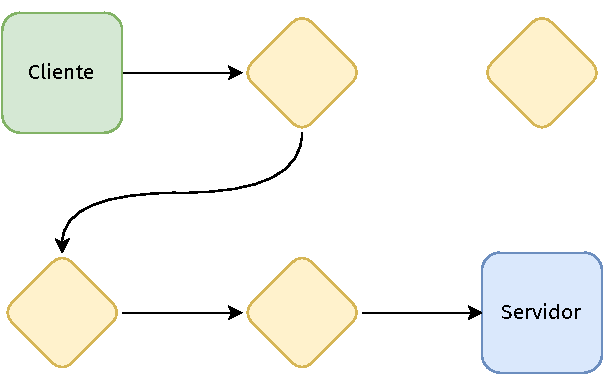
\includegraphics[width=0.5\textwidth]{images/crowds-protocol.pdf}
%	\end{figure}
%
%	\begin{itemize}
%		\item Una \emph{crowd} (multitud) de $N$ usuarios participa en el protocolo.
%		\item El cliente selecciona un usuario al azar.
%		\item Cada usuario selecciona probabilísticamente:
%		\begin{itemize}
%			\item Con probabilidad $p$ redirigir el mensaje a otro usuario.
%			\item Con probabilidad $1 - p$ enviar el mensaje al destino final (servidor).
%		\end{itemize}
%	\end{itemize}
%\end{frame}

\begin{frame}{\insertsection: Subasta}
	\begin{enumerate}
		\item Comprador envía oferta.
		\item Subastador:
			\begin{itemize}
				\item Vende artículo con probabilidad $\frac{1}{4}$
				\item Realiza contraoferta con probabilidad $\frac{3}{4}$.
			\end{itemize}
		\item Comprador:
			\begin{itemize}
				\item Vuelve a ofertar con probabilidad $\frac{2}{3}$.
				\item Abandona subasta con probabilidad $\frac{1}{3}$
			\end{itemize}
	\end{enumerate}
\end{frame}

\begin{frame}{\insertsection: Subasta}
	\begin{figure}
		\centering
		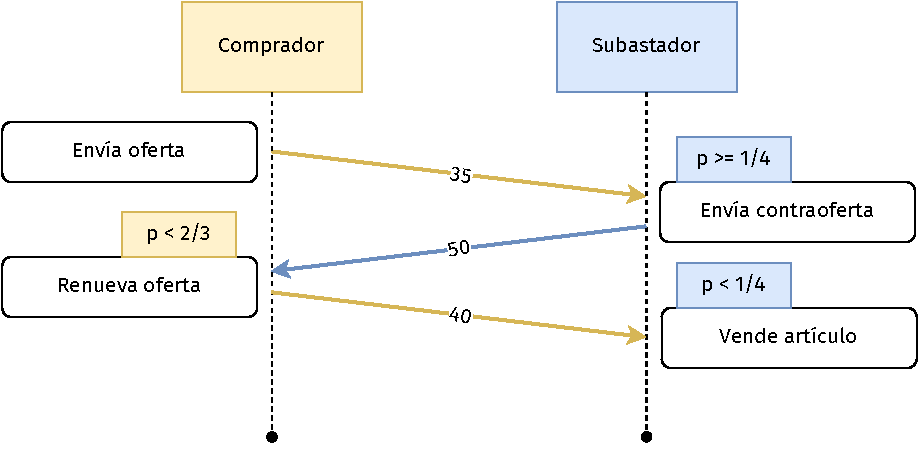
\includegraphics[width=0.9\textwidth]{images/auction-diagram.pdf}
		\caption{Ejemplo de subasta, $p \sim U(0, 1)$}
	\end{figure}
\end{frame}

\begin{frame}{\insertsection: Subasta}
	\AuctionBuyer[basicstyle=\footnotesize]
\end{frame}

\begin{frame}{\insertsection: Subasta}
	\Auctioneer[basicstyle=\footnotesize]
\end{frame}

\begin{frame}{\insertsection: Subasta}
	El tipo sesión que describe la interacción del Comprador es:
	\begin{equation*}
	    \label{eq:refined.auction}
	    \SessionType = \Out\tint{
		\BinaryPBranch[\frac{1}{4}]\Done{
		    \In\tint{
			\BinaryPChoice[\frac{2}{3}]\T\Idle
		    }
		}
	    }
	\end{equation*}

	Dado que no existe una interpretación universal de ``terminación
	exitosa'', se diferencia la terminación exitosa ($\Done$) de la
	infructuosa ($\Idle$) mediante constructores dedicados.

	\pause
	En este caso, la probabilidad de éxito (se concreta la venta) es de $\frac{1}{3}$.
\end{frame}

\section{Cambios a interfaz programática}

\begin{frame}[fragile]{\insertsection}

	\begin{table}[htb]
	    \begin{OCamlD}[basicstyle=\scriptsize,frame=single]
        val create  : unit -> $\etvar$ * $\sdual\etvar$
        val close   : $\End$ -> unit
        val send    : $\tvar$ -> $\Out\tvar\etvar$ -> $\etvar$
        val receive : $\In\tvar\etvar$ -> $\tvar$ * $\etvar$
        val select_true  : $\Choice\set{\Tag[True]: \etvarA}$ -> $\etvarA$
        val select_false : $\Choice\set{\Tag[False]: \etvarB}$ -> $\etvarB$
        val branch       : $\BinaryPBranch[]{\etvarA}{\etvarB}$ -> $\set{\Tag[True]: \etvarA,\ \Tag[False]: \etvarB}$
	    \end{OCamlD}
	\end{table}
\pause
	\begin{table}[htb]
	    \begin{OCamlD}[basicstyle=\scriptsize,frame=single]
        val create  : unit -> $\etvar$ * $\sdual\etvar$
        val close   : $\Done$ -> unit
        val idle    : $\Idle$ -> unit
        val send    : $\tvar$ -> $\Out\tvar\etvar$ -> $\etvar$
        val receive : $\In\tvar\etvar$ -> $\tvar$ * $\etvar$
        val select_true  : $\BinaryPChoice[1]{\etvarA}{\etvarB}$ -> $\etvarA$
        val select_false : $\BinaryPChoice[0]{\etvarA}{\etvarB}$ -> $\etvarB$
        val pick         : $p$ -> $(\BinaryPChoice[0]{\etvarA}{\etvarB}$ -> $\alpha)$
                             -> $(\BinaryPChoice[1]{\etvarA}{\etvarB}$ -> $\alpha)$
                             -> $\BinaryPChoice[p]{\etvarA}{\etvarB}$ -> $\alpha$
        val branch       : $\BinaryPBranch[p]{\etvarA}{\etvarB}$ -> $\set{\Tag[True]: \etvarA,\ \Tag[False]: \etvarB}$
	    \end{OCamlD}
	\end{table}
\end{frame}

\section{Elecciones probabilísticas}

\begin{frame}{\insertsection}
	TODO: contar qué se busca modelar con pick a nivel tipado
\end{frame}

\subsection{Elecciones multi-sesión}

\begin{frame}{\insertsubsection}
	TODO: Contar un poco qué son las elecciones multisesión y mostrar ejemplo que no tipa.
\end{frame}

\begin{frame}{\insertsubsection}
	TODO: Mencionar caminos posibles y solución utilizada
	\begin{figure}
		\centering
		\includegraphics[width=\textwidth]{images/pick-multi-sesión.png}
	\end{figure}
\end{frame}

\section{Composición de tipos sesión duales}

\begin{frame}{\insertsection}
	TODO: Introducir necesidad de representar el tipo "cerrado" para obtener la probabilidad de éxito. 
\end{frame}

\begin{frame}{\insertsection}
	TODO: Mostrar ejemplos de argumento opcional haciendo foco en que es puramente informativo.
\end{frame}

\subsection{Combinación multi-sesión}

\begin{frame}{\insertsubsection}
	TODO: Contar cómo se repite el mismo problema que con las elecciones multisesión
\end{frame}

\begin{frame}{\insertsubsection}
	TODO: Mencionar caminos posibles y solución utilizada
\end{frame}

\section{Probabilidad de éxito de una sesión}
\begin{frame}{\insertsection}
	TODO: Arrancar contando un poco del algoritmo para cálculo de probabilidad
\end{frame}

\subsection{Codificación de probabilidades}
\begin{frame}{\insertsubsection}
	TODO: Explicar cómo decidimos codificar las probabilidades para poder hacer el cálculo en tiempo de compilación. (codificación de enteros y racionales en el tipo)
\end{frame}

\section{Conclusión y trabajo a futuro}
\begin{frame}{\insertsection}
	TODO: Contar hasta dónde se llegó y qué mejoras se podrían hacer al sistema actual.
\end{frame}
